% CS F407 Artificial Intelligence: final project report.
% Format aligned strictly with project_report_template.tex (4-page extended limit).
\documentclass[11pt,a4paper,twocolumn]{article}

\usepackage[margin=2cm,columnsep=0.8cm]{geometry}
\usepackage[T1]{fontenc}
\usepackage{lmodern}
\usepackage{microtype}
\usepackage{amsmath,amssymb}
\usepackage{graphicx}
\usepackage{booktabs}
\usepackage{tabularx}
\usepackage{enumitem}
\usepackage{titlesec}
\usepackage{tikz}
\usetikzlibrary{shapes.geometric, arrows.meta, positioning, calc}
\usepackage{xurl}
\usepackage[hidelinks]{hyperref}

\titleformat{\section}{\normalsize\bfseries}{\thesection}{0.6em}{}
\titlespacing*{\section}{0pt}{1.2ex plus 0.3ex}{0.6ex}
\setlist{nosep,leftmargin=*}
\setlength{\parskip}{0.3ex}

\newcommand{\coursename}{CS F407 Artificial Intelligence, AY 2026--27 Semester I}
\newcommand{\teamno}{Team Syllogism}
\newcommand{\githuburl}{https://github.com/Arxalier/ChaturangZero}

\begin{document}

\twocolumn[{%
\begin{center}
  {\large\bfseries ChaturangZero: A Reinforcement Learning Agent to play Chaturanga}\\[1ex]
  \teamno\\
  Aaryan Pandey (2024A7PS0375G), Vraj Makwana (2024A7PS0606G),\\
  Harshal Lahoti (2024A7PS0870G), Sahaj Jhamb (2024A7PS0485G)\\[0.5ex]
  {\small \coursename, BITS Pilani, K.K. Birla Goa Campus}\\
  {\small \url{\githuburl}}\\[1.5ex]
  \begin{minipage}{0.85\textwidth}
    \small
    \centerline{\bfseries Abstract}\vspace{0.5ex}
    Chaturanga is an ancient Indian-origin board game with much more restrictive piece mobility compared to chess (for example, the queen can only move one step diagonally). Under these conditions, standard self-play reinforcement learning collapses into cyclic repetition draws, making learning from scratch ineffective without massive compute. To get around this problem, we developed ChaturangZero, pairing a dual-headed CNN with Polynomial Upper Confidence Trees (PUCT) Monte Carlo Tree Search. We found that training purely by self-play over 450 games left the model at par with uniform random play, as the value head got stuck outputting a near-constant evaluation. However, by deriving piece values from move mobility and training on a dataset of heuristic-backed games (about 10,000 greedy moves), the model improved significantly. The resulting agent consistently defeats random play with a 90.0\% win rate, and achieves an 87.5\% unbeaten rate (25.0\% wins, 62.5\% draws, 12.5\% losses) against four heuristic bots.
  \end{minipage}
\end{center}
\vspace{1.5ex}
}]

\section{Introduction}
Chaturanga is played on an $8 \times 8$ uncheckered grid called \emph{Ashtapada}~\cite{murray1913history,golombek1976chess}. While it is the ancestor of modern chess, its mechanics create a different ruleset:
\begin{enumerate}
    \item Foot Soldiers (\emph{Pad\={a}ti}) cannot double-step on turn one.
    \item Ministers (\emph{Mantri}) move only one step diagonally.
    \item Elephants (\emph{Gaja}) strictly leap two squares diagonally.
    \item Pawns promote exclusively to Ministers upon reaching the back rank.
    \item Capturing all opponent non-king pieces (\emph{Bare King}) triggers an immediate win.
    \item Stalemate counts as an outright win for the stalemated player.
\end{enumerate}

These restrictions cause extreme game lengths. In random play, the median game lasts 411 plies. When AlphaZero-style self-play is attempted with limited compute, both players rarely engage before hitting repetitive moves. Because games run so long, the agent rarely sees a win or loss signal, and both the policy and value heads fail to learn.

\subsection{Input and Output Specification}
\begin{itemize}
    \item \textbf{Input}: A $(13, 8, 8)$ binary tensor encoding the board for 6 piece types per player and a constant turn plane.
    \item \textbf{Output}: A 4,096-dimensional masked legal policy vector $\boldsymbol{\pi} \in \mathbb{R}^{4096}$ and a scalar position evaluation $v \in [-1, +1]$.
\end{itemize}

\subsection{Contributions}
\begin{enumerate}
    \item We implemented an end-to-end ancient Chaturanga engine, web UI, and dual-headed ResNet paired with PUCT MCTS.
    \item We showed why training purely from scratch fails due to endless repetition draws.
    \item We introduced a first-principles derivation method for heuristics, calibrated with human feedback, to bootstrap the network. By bootstrapping the method, we mean to supply it with training data of games played with greedy rules so it can learn the intrinsic value of pieces. It is worth noting that this violates the condition of the bot learning purely through self-play. Despite this, we wanted to see how well the bot can perform with some pre-trained insights.
    \item We evaluated the agent against random play, four Scholar minimax bots, a 900-game round-robin Elo suite, and ablations.
\end{enumerate}

\section{Background and related work}

\subsection{AlphaZero and PUCT Search}
AlphaZero replaces evaluation functions with a deep neural network $f_\theta(s) = (\mathbf{p}, v)$ trained through reinforcement learning from self-play~\cite{silver2018alphazero}. In each turn, Monte Carlo Tree Search (MCTS) uses a four step process to evaluate the game's search tree (Figure~\ref{fig:mcts_stages}), using network priors $\mathbf{p}$ and scalar values $v$ to guide tree expansion via Polynomial Upper Confidence Trees (PUCT):
\begin{equation}
\text{PUCT}(s, a) = Q(s, a) + c_{\text{puct}} \cdot P(s, a) \cdot \frac{\sqrt{N(s)}}{1 + N(s, a)}
\end{equation}

\begin{figure}[t]
\centering
\resizebox{0.62\columnwidth}{!}{%
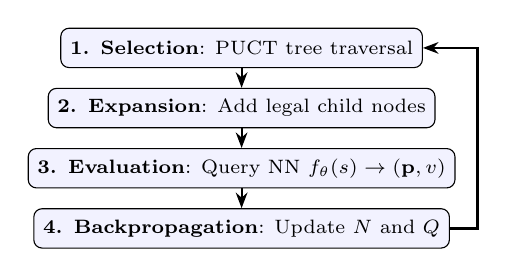
\begin{tikzpicture}[
    stage/.style={draw, rectangle, rounded corners=3pt, minimum width=3.4cm, minimum height=0.5cm, text centered, font=\scriptsize, fill=blue!5},
    arrow/.style={-{Stealth[scale=0.85]}, thick}
]
    \node[stage] (s1) at (0, 0) {\textbf{1. Selection}: PUCT tree traversal};
    \node[stage, below=0.25cm of s1] (s2) {\textbf{2. Expansion}: Add legal child nodes};
    \node[stage, below=0.25cm of s2] (s3) {\textbf{3. Evaluation}: Query NN $f_\theta(s) \to (\mathbf{p}, v)$};
    \node[stage, below=0.25cm of s3] (s4) {\textbf{4. Backpropagation}: Update $N$ and $Q$};
    \draw[arrow] (s1) -- (s2);
    \draw[arrow] (s2) -- (s3);
    \draw[arrow] (s3) -- (s4);
    \draw[arrow] (s4.east) -- ++(0.35,0) |- (s1.east);
\end{tikzpicture}%
}
\caption{The four iterative stages of MCTS.}
\label{fig:mcts_stages}
\end{figure}

\subsection{Deep Reinforcement Learning in Board Games}
Modern game-playing agents rely on policy iteration where MCTS acts as a policy improver~\cite{silver2017alphago}. However, tabular and deep actor-critic methods struggle when reward signals are delayed over hundreds of steps~\cite{dash2026deeprl}. While multi-variant classical engines like Fairy-Stockfish can be configured to play Chaturanga using alpha-beta search~\cite{russell2021aima}, there are no deep reinforcement learning counterparts (like AlphaZero for Chess). We aim to bridge that gap by modeling an AlphaZero-like architecture over the base rules of ancient Chaturanga.

\section{Method}

\subsection{Board Encoding and Neural Architecture}
The board is converted into 13 binary feature planes: channels 0--5 for White $P, H, E, R, M, K$, channels 6--11 for Black $P, H, E, R, M, K$, and channel 12 as a turn indicator ($1.0$ for White, $0.0$ for Black). The action space maps all from-square to to-square transitions:
\begin{equation}
\text{action} = (r_{\text{start}} \times 8 + c_{\text{start}}) \times 64 + (r_{\text{end}} \times 8 + c_{\text{end}})
\end{equation}

\begin{figure}[t]
\centering
\resizebox{0.76\columnwidth}{!}{%
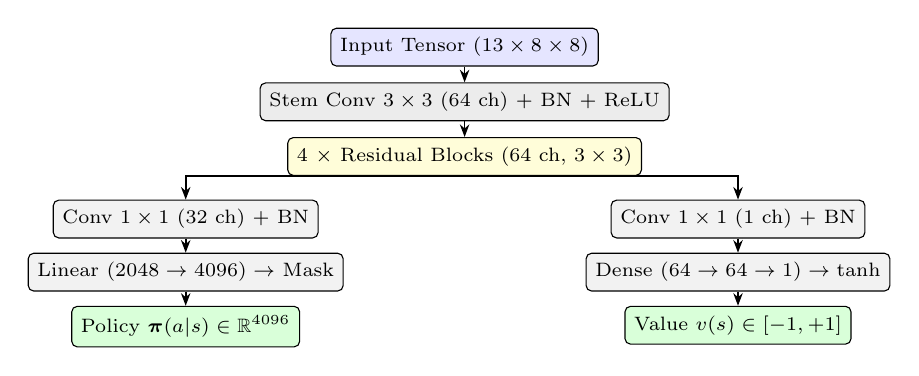
\begin{tikzpicture}[
    box/.style={draw, rectangle, rounded corners=2pt, minimum height=0.45cm, text centered, font=\scriptsize},
    headbox/.style={draw, rectangle, rounded corners=2pt, minimum height=0.45cm, text centered, font=\scriptsize, fill=gray!10},
    arrow/.style={-{Stealth[scale=0.8]}, semithick}
]
    \node[box, fill=blue!10] (input) at (0, 0) {Input Tensor $(13 \times 8 \times 8)$};
    \node[box, fill=gray!15, below=0.2cm of input] (conv0) {Stem Conv $3\times3$ (64 ch) + BN + ReLU};
    \node[box, fill=yellow!15, below=0.2cm of conv0] (res) {4 $\times$ Residual Blocks (64 ch, $3\times3$)};
    \node[headbox, below left=0.3cm and -0.4cm of res] (pol_conv) {Conv $1\times1$ (32 ch) + BN};
    \node[headbox, below=0.18cm of pol_conv] (pol_lin) {Linear $(2048 \to 4096) \to$ Mask};
    \node[box, fill=green!15, below=0.18cm of pol_lin] (pol_out) {Policy $\boldsymbol{\pi}(a|s) \in \mathbb{R}^{4096}$};
    \node[headbox, below right=0.3cm and -0.4cm of res] (val_conv) {Conv $1\times1$ (1 ch) + BN};
    \node[headbox, below=0.18cm of val_conv] (val_lin) {Dense $(64 \to 64 \to 1) \to \tanh$};
    \node[box, fill=green!15, below=0.18cm of val_lin] (val_out) {Value $v(s) \in [-1, +1]$};
    \draw[arrow] (input) -- (conv0);
    \draw[arrow] (conv0) -- (res);
    \draw[arrow] (res.south) -| (pol_conv.north);
    \draw[arrow] (res.south) -| (val_conv.north);
    \draw[arrow] (pol_conv) -- (pol_lin);
    \draw[arrow] (pol_lin) -- (pol_out);
    \draw[arrow] (val_conv) -- (val_lin);
    \draw[arrow] (val_lin) -- (val_out);
\end{tikzpicture}%
}
\caption{Dual-headed Convolutional ResNet architecture.}
\label{fig:cnn_arch}
\end{figure}

The backbone uses an initial $3 \times 3$ conv (64 filters, 7,616 params) and 4 residual blocks (295,936 params). The policy head uses a $1 \times 1$ conv (32 ch) and dense projection ($2048 \to 4096$, 8,394,848 params) masking illegal moves to $-\infty$; the value head uses a $1 \times 1$ conv (1 ch), two dense layers ($64 \to 64 \to 1$, 4,292 params), and $\tanh$ (8,702,692 params total).

\subsection{Why Pure Self-Play Underperformed}
Our initial attempt used pure self-play over 30 iterations (15 games/iter, 450 games total, 20 MCTS sims/move). Training failed due to two factors:
\begin{enumerate}
    \item \textbf{Horizon Length}: Players require 30--50 plies simply to cross the board. Pawns cannot leap forward, and ministers cover only 32 squares.
    \item \textbf{Repetition Cycles}: With an untrained value head, MCTS drifted into cyclic piece shuffling, ending in 3-fold repetition draws by ply 45.
\end{enumerate}
With over 90\% of games drawing ($z = 0$), the value head froze near $+0.133$ everywhere, leaving MCTS unable to distinguish captures.

\subsection{Deriving Piece Values from Move Mobility}
At this point, we decided to experiment instead of concluding. While we could not train purely through self-play, we wanted to see how well our architecture could perform with external help. Instead of guessing piece weights by hand, \texttt{discover\_values.py} estimates them from move rules:
\begin{equation}
\mathbb{E}[M_p] = \frac{1}{64} \sum_{r=0}^{7} \sum_{c=0}^{7} |\text{moves}(p, r, c)|
\end{equation}
Across an empty Ashtapada, average reaches are $1.64$ (Pawn, base), $2.25$ (Elephant), $3.06$ (Minister), $5.25$ (Horse), and $14.00$ (Chariot). Applying sublinear dampening ($\alpha = 0.85$) for slider obstruction, $V_{\text{raw}}(p) = (\mathbb{E}[M_p]/\text{base})^{0.85}$, gives Pawn $1.00$, Elephant $1.31$, Minister $1.70$, Horse $2.69$, and Chariot $6.19$, alongside a min-max $[0.00, 0.20]$ central $4 \times 4$ bonus.

\subsection{Manual Calibration and Supervised Bootstrapping}
We adjusted these numbers slightly by hand for early crowding:
\begin{equation}
\mathbf{w}_{\text{aligned}} = [P{:}1.0, \, E{:}1.5, \, M{:}2.0, \, H{:}3.0, \, C{:}5.0]
\end{equation}
We generated 150 curriculum games using 2-ply teacher evaluations ($\epsilon = 0.15$) and fine-tuned for 12 epochs:
\begin{equation}
\mathcal{L} = 4.0 \cdot (z - v)^2 - \boldsymbol{\pi}^\top \log \mathbf{p} + c \|\theta\|^2
\end{equation}
Value loss dropped from $0.1752$ to $0.0099$, and policy loss dropped from $2.7178$ to $0.2218$.

\section{Experimental setup}
\textbf{Baselines}: Uniform Random Bot; NoviceBot (80\% random, 20\% greedy capture); and three depth-2 alpha-beta bots---ChanakyaBot (material/checks/bare-king), AryabhataBot (piece-square centrality tables), and PaniniBot (defense/king shelter). Arena runs also test Greedy 1-ply and Minimax depth-2.
\textbf{Hardware}: Local runs used an Intel x86\_64 CPU (16 logical cores, PyTorch 2.6, single-thread inference to avoid OpenMP contention); arena sweeps ran on Apple M3.

\section{Results}

\subsection{Material Valuation Diagnostic Probe}
Table~\ref{tab:probe} shows value-head evaluations when White is up or down a piece from the start board. Evaluations move monotonically in the right direction for every piece type, with Horses and Chariots causing the largest swings.

\begin{table}[h]
\centering
\small
\resizebox{\columnwidth}{!}{%
\begin{tabular}{lccc}
\toprule
Piece Configuration & White Adv. & White Disadv. & Net Delta \\
\midrule
Pawn (\emph{Pad\={a}ti}) & +0.0589 & -0.0213 & \textbf{+0.0803} \\
Elephant (\emph{Gaja}) & +0.0611 & -0.0773 & \textbf{+0.1383} \\
Minister (\emph{Mantri}) & +0.0794 & -0.0146 & \textbf{+0.0939} \\
Horse (\emph{Ashwa}) & +0.3545 & -0.1142 & \textbf{+0.4687} \\
Chariot (\emph{Ratha}) & +0.2340 & -0.2410 & \textbf{+0.4750} \\
Major (+Ratha +Ashwa) & +0.5748 & -0.3850 & \textbf{+0.9598} \\
\bottomrule
\end{tabular}%
}
\caption{Value Head material diagnostic probe matrix.}
\label{tab:probe}
\end{table}

\subsection{Benchmark vs. Uniform Random Bot}
Table~\ref{tab:random_bench} evaluates 10 games against Uniform Random play. At 200 sims, the agent converts games in an average of 144 plies until it bares the opponent's king.

\begin{table}[h]
\centering
\small
\resizebox{\columnwidth}{!}{%
\begin{tabular}{lccccc}
\toprule
Training Regime & Sims & Plies & AI Win & Rand Win & Draw \\
\midrule
Pure Self-Play (30 iters) & 20 & 120 & 0.0\% (0) & 10.0\% (1) & 90.0\% (9) \\
Bootstrapped Fine-Tune & 40 & 300 & 90.0\% (9) & 0.0\% (0) & 10.0\% (1) \\
Bootstrapped Fine-Tune & 200 & 250 & \textbf{90.0\% (9)} & \textbf{0.0\% (0)} & \textbf{10.0\% (1)} \\
\bottomrule
\end{tabular}%
}
\caption{Benchmark results vs. Uniform Random Bot (10 games).}
\label{tab:random_bench}
\end{table}

\subsection{Tournament Benchmark vs. Scholar Bots}
We pitted the trained agent against the four Scholar bots in an 8-game tournament (1 White, 1 Black per bot, cutoff 260 plies, Table~\ref{tab:tourney}). It reached an 87.5\% unbeaten rate (25.0\% wins, 62.5\% draws, 12.5\% losses), defeating NoviceBot twice and holding ChanakyaBot and AryabhataBot to draws.

\begin{table}[h]
\centering
\small
\resizebox{\columnwidth}{!}{%
\begin{tabular}{lcccc}
\toprule
Opponent & AI Wins & Bot Wins & Draws & AI Win Rate \\
\midrule
NoviceBot & 2 & 0 & 0 & \textbf{100.0\%} \\
ChanakyaBot & 0 & 0 & 2 & 0.0\% (100\% draw) \\
AryabhataBot & 0 & 0 & 2 & 0.0\% (100\% draw) \\
PaniniBot & 0 & 1 & 1 & 0.0\% (50\% draw) \\
\midrule
\textbf{Total} & \textbf{2 (25.0\%)} & \textbf{1 (12.5\%)} & \textbf{5 (62.5\%)} & \textbf{25.0\%} \\
\bottomrule
\end{tabular}%
}
\caption{Tournament benchmark against heuristic Scholar Bots.}
\label{tab:tourney}
\end{table}

\subsection{Round-Robin Arena, Elo Tiers, and Ablations}
A 10-player round robin in \texttt{arena/} (900 games, Bradley--Terry Elo anchored at Random $= 0$) ranked \texttt{AZ-Master} (80 sims, $\tau{=}0.05$) at \textbf{499 Elo} (60.3\%), ahead of \texttt{Greedy-1ply} (429), \texttt{AZ-Intermediate} (15 sims, 275), \texttt{AZ-Novice} (152), and \texttt{NoviceBot} (149), while trailing depth-2 minimax (\texttt{Aryabhata} 608, \texttt{Panini}/\texttt{Chanakya} 618, \texttt{Minimax-d2} 672). Ablations confirmed: 93.7\% of random rollouts fail to finish within 120 plies (0.56 correlation at 40.8\,ms vs.\ 0.77 at 1.6\,ms for the value head), unmasked softmax puts 99.5--100\% mass on illegal moves (7.2\% vs.\ 14.6\% accuracy), and 1-ply greedy play falls into Elephant-leap traps 48.5\% of the time vs.\ 10.0\% for 80-sim MCTS.

\section{Discussion and limitations}
\textbf{The Draw Tendency}: 62.5\% of games against heuristic bots ended in 3-fold repetition draws because: (1) Scholar bots lack move history and oscillate between equal evaluations; and (2) $V(s) \approx 0.0$ makes MCTS treat repetition draws identically to equal positions (allowing a draw at ply 112 in Game 6 vs.\ AryabhataBot even with 8 vs.\ 4 pieces).

\textbf{Search Depth, Model Size, and Compute}: \texttt{ChaturangaNet} has 8.70M parameters (96.4\% in the dense $2048 \to 4096$ policy layer). Slow sequential passes limited pure RL to 450 games, too little data for that capacity. At 30 sims, MCTS only searches 1--2 plies deep and falls into depth-2 traps; 300 sims plays stronger but needs $\sim$30,000 passes per game (4--5 min on CPU).

\textbf{Future Work}: (1) A smaller CNN (a few thousand params, convolutional policy head) to train over thousands of games quickly; (2) a contempt factor ($V = -0.25$) on repetitions when ahead; (3) GPU batched MCTS for sub-10s games.

\section{Conclusion}
We built ChaturangZero, a neural MCTS agent for ancient Chaturanga. We showed that pure self-play from scratch fails in low-mobility board games due to extreme game horizons and draw collapse. Bootstrapping from mobility heuristics lifted wins vs.\ random play from 0\% to 90\%, reached an 87.5\% unbeaten rate vs.\ depth-2 Scholar bots, and scored 499 Elo in a 900-game arena.

\section*{Individual member contributions}
{\small
\begin{tabularx}{\linewidth}{@{}l X@{}}
\toprule
Name & Contribution \\
\midrule
\textbf{Aaryan Pandey} & Training pipeline lead: MCTS-NN integration, self-play loop, curriculum, bootstrapping, loss masking. \\
\textbf{Vraj Makwana} & Deep learning architect: Board-to-tensor encoder, action indexing, 4-block dual-headed ResNet. \\
\textbf{Sahaj Jhamb} & Heuristic engine: Scholar bots (Novice, Chanakya, Aryabhata, Panini) and baseline testing. \\
\textbf{Harshal Lahoti} & Web UI \& arena: Interactive board UI, 900-game round-robin Elo suite, skill tiers, ablations. \\
\bottomrule
\end{tabularx}}

\smallskip
\noindent All members have read this report and agree with the statement above.

\section*{Generative AI disclosure}
Generative AI tools were used during this project as follows: \textbf{Gemini 3.8 Flash \& Gemini Neon} for drafting unit tests, debugging tensor action masking, and formatting tables; \textbf{Claude Opus 5} for code review, mobility math validation, and frontend UI. All code and report text were manually verified, debugged, and tested by the team.

\section*{Code availability}
\noindent Code and data:\\
\url{\githuburl}\\
The public repository contains source code, trained weights, evaluation logs, and README instructions to reproduce the results reported here.

\begin{thebibliography}{9}
\small
\bibitem{silver2018alphazero}
D.~Silver, T.~Hubert, J.~Schrittwieser, et~al.
\newblock A general reinforcement learning algorithm that masters chess, shogi, and Go through self-play.
\newblock \emph{Science}, 362(6419):1140--1144, 2018.

\bibitem{silver2017alphago}
D.~Silver, J.~Schrittwieser, K.~Simonyan, et~al.
\newblock Mastering the game of Go without human knowledge.
\newblock \emph{Nature}, 550(7676):354--359, 2017.

\bibitem{dash2026deeprl}
T.~Dash.
\newblock Deep Reinforcement Learning.
\newblock Lecture Slides, CS F407 Artificial Intelligence, BITS Pilani, AY 2025--26 Sem II.
\newblock \url{https://github.com/tirtharajdash/CS-F407-AI-AY2025-26-S2/blob/main/lectures/deep_rl.pdf}.

\bibitem{russell2021aima}
S.~Russell and P.~Norvig.
\newblock \emph{Artificial Intelligence: A Modern Approach}, 4th edition.
\newblock Pearson, 2021.

\bibitem{murray1913history}
H.~J.~R. Murray.
\newblock \emph{A History of Chess}.
\newblock Oxford University Press, 1913.

\bibitem{golombek1976chess}
H.~Golombek.
\newblock \emph{Chess: A History}.
\newblock G.~P. Putnam's Sons, 1976.
\end{thebibliography}

\end{document}
